\documentclass[12pt,twoside]{report}
\usepackage[a4paper,width=150mm,headheight=110pt,top=25mm,bottom=25mm]{geometry}
\usepackage[utf8]{inputenc}
\usepackage{listings}
\usepackage{graphicx}
\usepackage{tikz}
\usepackage{pgffor} 
\usepackage{float}
\usepackage{graphics} 
\usepackage{fancyhdr}
\usepackage[round, numbers,authoryear]{natbib}
\usepackage{color}
\usepackage{indentfirst}
\usepackage{epigraph}
\usepackage{ragged2e}
\usepackage{blindtext}
\graphicspath{{images/}}

\definecolor{mycolor}{RGB}{30,75,180}
\definecolor{mycolor2}{RGB}{40,75,90}
\definecolor{red}{RGB}{200,0,0}
\usepackage[colorlinks = true,
            linkcolor = mycolor,
            urlcolor  = mycolor,
            citecolor = mycolor,
            anchorcolor = mycolor]{hyperref}

\usepackage[hypcap=true,font={small,it}]{caption}
\usetikzlibrary{calc}

\captionsetup{belowskip=2pt,aboveskip=2pt}
\bibliographystyle{abbrvnat}

\renewcommand{\chaptername}{}

\renewcommand{\figureautorefname}{figure} % lower case default ref
\renewcommand{\tableautorefname}{table} % lower case default ref
\newcommand{\latex}{\LaTeX\xspace}
\newcommand{\mcite}[1]{\textcolor{mycolor}{\citeauthor{#1} (\citeyear{#1})}}
\newcommand{\hcite}[1]{(\textcolor{mycolor}{\citeauthor{#1}, \citeyear{#1}})}
\newcommand{\defi}[1]{\textbf{#1}}
\newcommand{\naming}[1]{\textbf{#1}}
\newcommand{\todo}[1]{\textbf{\color{red} TODO: #1}}
%----------------------------------------------------------------------------------------------------%

%--------------------------------------------- DOCUMENT ---------------------------------------------%
\begin{document}
%\fancyhead[RO,LE]{}

% Title page
    \begin{titlepage}
\vspace*{-2.5cm}
\begin{figure}[H]
    \hspace*{-1.0cm}
    \vspace*{-0.5cm}
    
\includegraphics[scale=0.4]{images/logo_ime.png}\\
\end{figure}

\noindent Universidade de São Paulo - Instituto de Matemática e Estatística\\
Bachelor's Programme in Computer Science
    \begin{center}
        \vspace*{1cm}
        
        {\LARGE \textbf{HOT GAMES}}
        
        \vspace{0.5cm}
        Temperature, advantage and numbers
        
        \vspace{1.5cm}
        by \\
        \vspace{1.5cm}
       Matheus Tararam de Laurentys
                
        \vspace{1.0cm}
    \end{center}

\noindent{
\textcolor{red}{{\bf Abstract} (The Abstract is a short summary of what your thesis is about. It accurately reflects the content of the thesis providing information about the research problem, research aims, methods and procedures, results and implications. It is a short section. Abstracts give readers the opportunity to quickly see the main contents of the paper and enable them to decide whether the paper is of particular interest to their needs. This section will be one of the last sections that you write. No subheadings are used in an abstract.)
}
}
\vfill
\textcolor[rgb]{0.5,0.5,0.5}{
    \begin{flushleft}
    { \small
    MAC0499 \\
    Undergraduate Thesis \\
    (Month) (Year) \\
    Supervisor: José Coelho Pina \\
    }
    \end{flushleft}
}
      
\end{titlepage}

% Optional Chapters

    %\chapter*{Dedication}
    %\chapter*{Declaration}
    \chapter*{Acknowledgements}
    \textcolor{red}{It is usual, but not compulsory, to thank those who have been of particular help to you in completing the thesis.}

% Table of contents, list of figures, and list of tables
    {\hypersetup{linkcolor=black}
        \tableofcontents
        \listoffigures
        \listoftables
    }
        {\hypersetup{linkcolor=mycolor}}
    
% Introduction
    \chapter{Introduction} 
    \renewcommand{\textflush}{flushepinormal}
\setlength\epigraphwidth{.8\textwidth}
\epigraph{``I learned very quickly that playing games and working on mathematics were closely intertwined activities for him, if not actually the same activity. His attitude resonated with and affirmed my own thoughts about math as play, though he took this attitude far beyond what I ever expected from a Princeton math professor, and I loved it."}{Manjul Bhargava \footnotemark}

\footnotetext{Fields medalist commenting on John Horton Conway's passing}



It is no surprise that avid players of games that resemble logical or
mathematical puzzles, like checkers, develop an intuition that allows
them to calculate faster. This intuition comes in many forms like
asserting bad moves fast and recognizing losing, drawing and winning
patterns. A most essential, and sometime very hard, component of
playing well any of these mathematical games is being able to know if
you are ahead or behind in a given position.

%%%%%%%%%%%%%%%%%%%%%%%%%%%%%%%%%%%%%%%%%%%%%%%%%%%%%%%%%%%%%%%%%%%
% mensagem caso 1 jogo não é suficiente para caso n jogos
%%%%%%%%%%%%%%%%%%%%%%%%%%%%%%%%%%%%%%%%%%%%%%%%%%%%%%%%%%%%%%%%%%%
While asserting which player a position favors is already a hard task,
this ability is not enough to play well in the games this text
showcases. Consider the following variant of the game of chess: each
player is given a set of board positions, and each should choose one
board to play as white. During this game, play will take place in each
board in parallel, and, whoever checkmates the opponent faster, wins
the game. If one wants to be a great player of this variant, asserting
if a position is winning or loosing in a regular chess game is not
enough, nor is the ability to play regular chess perfectly.

The most important ability for this ``parallel'' variant, 
and for the games that this text focus on, is
to score each position.
%%%%%%%%%%%%%%%%%%%%%%%%%%%%%%%%%%%%%%%%%%%%%%%%%%%%
Scoring a position is different from spotting which one
is better from a range of options.
%%%%%%%%%%%%%%%%%%%%%%%%%%%%%%%%%%%%%%%%%%%%%%%%%%%
To simplify, for these first few pages, the reader can
regard scoring as labeling a position with a real number.
%%%%%%%%%%%%%%%%%%%%%%%%%%%%%%%%%%%%%%%%%%%%%%%%%%%%%%%
If one can label different position in chess, and
these labels reflect advantage, 
then playing the proposed variation becomes easy.
%%%%%%%%%%%%%%%%%%%%%%%%%%%%%%%%%%%%%%%%%%%%%%%%%%%%%
In this day and age, making a 
classifier that performs well is chess,
or the proposed variant, and
many other games of this sort is a reality.
%%%%%%%%%%%%%%%%%%%%%%%%%%%%%%%%%%%%%%%%%%%%%%%%%%%%%%%%%%%%
However, a method to perfectly classify, or at least proving
a position is better than another, is not widespread.
 
The ability to precisely calculate the advantage a player has in a
position is the object of interest of Combinatorial Game Theory.
%%%%%%%%%%%%%%%%%%%%%%%%%%%%%%%%%%%%%%%%%%%%%%%%%%%%%%%%%%%%%%%%
This theory provides means of labeling all positions in games, not
just in chess, but in all combinatorial games.
%%%%%%%%%%%%%%%%%%%%%%%%%%%%%%%%%%%%%%%%%%%%%%%%%%%%%%%%%%%%
A position in Go and a position Checkers, two different games,
might have the same label and that means they are both equally
good or bad. The modern approach to combinatorial games
was inaugurated in~1976 in the book
\textit{On Numbers And Games}\cite{ONAG1}, but there are studies that date
back from the 1930s~\cite{CGT}.
%%%%%%%%%%%%%%%%%%%%%%%%%%%%%%%%%%%%%%%%%%%%%%%%%%%%%%%%%%%%
The author of that book, Jonh Horton Conway, as
found in the epigraph that starts this text, was, as many, an avid
player of such games.
%%%%%%%%%%%%%%%%%%%%%%%%%%%%%%%%%%%%%%%%%%%%%%%%%%%%%%%%%
In fact, Conway tells that the event that led to
him invent, or discover, this theory was watching two Go players
playing an endgame.

Conway realized that some positions
behaved like numbers, in every aspect.
%%%%%%%%%%%%%%%%%%%%%%%%%%%%%%%%%%%%%%%%%%%%%%%%%%%%%%%%%%
While, initially, that seems very useful to evaluate games,
Conway went ahead and proposed that some positions \textbf{are}
numbers.
%%%%%%%%%%%%%%%%%%%%%%%%%%%%%%%%%%%%%%%%%%%%%%%%%%%%%%%%%%
There is a  difference between label an object
as a number and an the object \textit{being} that number.
%%%%%%%%%%%%%%%%%%%%%%%%%%%%%%%
The key point in Conway's ideia is
that one can define operations as addition
such that the sum of two games
\textit{is} the sum of the numbers they are equal to.
%%%%%%%%%%%%%%%%%%%%%%%%%%%%%%%
The beautiful thing about games is that the sum is defined
in the most natural way.
%%%%%%%%%%%%%%%%%%%%%%%%%%%%%%%%%%%%%%%%%%%%%%%%%%%%%%%%%%%%
PARAMOS AQUI
%%%%%%%%%%%%%%%%%%%%%%%%%%%%%%%%%%%%%%%%%%%%%%%%%

%%%%%%%%%%%%%%%%%%%%%%%%%%%%%%%%%%%%%%%%%%%%%%%%%%%%%%%%%%
Later the reader will be presented to the  idea that
integer numbers are games, fractions are games, reals are games,
and many more numbers are also games.
%%%%%%%%%%%%%%%%%%%%%%%%%%%%%%%%%%%%%%%%%%%%%%%%%%%%%%%%%
This match is further explained in the
following chapters and is the main topic in this
field of study.

As stated before, there are games that are numbers, but not real. In fact the games that are numbers formed a new set, to be analyzed in the next sections. These numbers will not look like numbers at first. However, after visiting how they add up together in the most natural way, how they form an enormous set from extremely simple rules and other great characteristics, like being a completely ordered set, the reader might start appreciating them. The Surreal Numbers\footnote{Originally Conway only called them numbers, but greatly appreciated the name given by Knuth}, name given by Donald Knuth in \textit{Surreal Numbers: How Two Ex-Students Turned on to Pure Mathematics and Found Total Happiness}\cite{SN}.

As some might understand from the title alone, however, the focus of this text are in the non-numbers. It is possible for games to not behave like any of the surreal numbers, although every surreal number has correspondent\footnote{There are infinite games that are equal to any Surreal Number} games. The concept of temperature, and by consequence all the simpler concepts like hotness and coolness, however, does not forego the understanding of numbers. The reader will find that all games become numbers after some moves, so understanding them is paramount.

After a vista on both numbers and non-numbers, this text has two chapters targeted on exercising the concepts learned, visiting fun games to play and proofs on classes of games, including a new result from 2019 which is the first of its kind. The text as a whole will make the case that Combinatorial Game Theory is built upon extremely simple but powerful concepts. The few concepts are considered powerful because they not only provide a vast field of problems but allow simple proofs for them as well.

The next three sections will present the basics of Combinatorial Game Theory, describing numbers and non-numbers. The style of these sections will be similar to that of the book \textit{Winning Ways for your Mathematical Plays}\cite{WW}. It means that concepts, notation and theorems are not highlighted or enumerated and, instead, their meaning are presented in the regular paragraphs. This style fits well a text in Combinatorial Game Theory because most most of them are extremely simple and only a few of them are abstract. In this field, it is easy to write examples of the concepts so there is no necessity of abstracting as much as other areas of algebra or combinatorics.

The style of the book is also widely known for being non-rigorous where it does not have to be. The book will commonly use images of games that satisfy assertion and provide, or not, a logic why other games also satisfy that, without a rigorous proof. This is not followed as much in this text, justifications may be provided where not required. 

On the other side of the spectrum there is \textit{Combinatorial Game Theory}\cite{CGT}. Siegel is likely the most active researcher of the field nowadays and created the most developed tool used to analyze them, CGSuite. CGSuite is an very useful tool and more about it may be found in appendix A. Unlike the authors of \textit{Winning Ways for your Mathematical Plays}, he gave a great deal of form to this field. The book contains hundreds of definitions, notations, theorems and lemmas which are all enumerated and highlighted. One of the results is that his standards became widely used and that helps reading current papers. In general the book is more advanced and is the primary reference for chapters 5 and 6.

Between the two there is the book \textit{On Numbers and Games}\cite{ONAG1}\cite{ONAG2}, and possibly all others. The first edition of the book, as stated before, gave birth to the modern approach of Combinatorial Game Theory. The book is much more theoretic and focused on pure mathematics, containing much more algebra and number theory, than the successors, but is also extremely descriptive. There are other great books, but almost all the content of this text references only these three books.

Lastly, it may be worth observing that the text does not, nor does it intend to, contain everything there is in the field. In fact, it does not even shows everything there is about hot games. It may, however, serve as reference to short partisan games and will bring all the fundamental concepts of this class of games. There is a list of content that was omitted and approaches that were not discussed in the final chapter. Notice, however, that short games form a massive class of games and many of the fun games are short, so studying them first is typical, and hopefully it sparks interest in the remaining areas of the field.














    
% Definitions
    \chapter{What to do with Pen, Paper and a Friend}
    %\chapter{Pen, Paper, a Friend and the Rules}
    
In order to study mathematical plays and answer the many questions they raise a new mathematical field of study was developed and many new terms were created. The phrase "mathematical play" is in itself a new term, for instance. While the most common term is "Combinatorial Games", the canonical reference for this field \textit{Winning Ways for Your Mathematical Plays} 1981, uses the former, not the latter. As more is said about the topic, more meaning the term "mathematical play" is going to acquire.

The name ``Combinatorial Game" might bring to light some information. It, at least, means that this field will deal with games, as in, an instance of a Game Theory problem, and, more specifically, a subset of those games. It also brings to light that the use of counting, finite structures and, most likely, graph representations will be heavily used (combinatorics). However, a definition of the object of interest becomes possible with the name mathematical play.

To play something mathematical could be understood as to engage in an activity in which the better use of mathematical ability, such as counting and logic, would result in advantage over its poor use. However it could be detailed further to an activity in which mathematical ability is the single defining factor. The later might make more sense because there are games, like poker, that do require some counting ability; however, luck and reading behavior skill are much more valuable to a successful game and this is something the definition would be better off forbidding.

\defi{Chance moves}, like throwing a dice or flipping a card, are not fit for mathematical plays. Even with their removal, however, there are possibilities that would not me comfortably called mathematical plays. The nature of a mathematical plays is that both players can engage the same activity and generate advantages out of "good play". For instance, it would be hard to agree that two people play rock-paper-scissors are battling a mathematical fight (even though there are no chance moves).

It is very important that all players have \defi{complete information} of the position. Games like rock-paper-scissors, in which players take action simultaneously, block complete information. Therefore, players must \textbf{move alternately}. The last concerning factor in discerning mathematical from non-mathematical plays during this analysis is the number of players.

When each player has more than one opponent a greater goal (than gaining advantage) arises. When playing with over two people it is frequent that the best move is not the one that brings  a better position but one that prevents any of the opponents from gaining an winning advantage. While that can be very mathematical, there is a clear distinction between sticking to two player games and allowing any number of players (notice that one can consider soccer as a two player game - even though there are multiple agents in a team). In order to focus on the mathematical ability to make the best move, the option to allow only \textbf{two players} is the most interesting.

The only remaining criteria of this definition (as established in [\todo{WW}]), that is related to the term play, and not the term mathematical, is preventing an infinite game. The rules of the game must guarantee that from any starting position, \defi{\todo{play should always} end because a player will not have moves available}. If following "\defi{normal play}" convention, a player that cannot move is lost. It is  correct to assume normal play, unless specified otherwise, in this field of study.

The foundations of mathematical plays, highlighted, give light to a complex and rich set of problems. At the same time, some other complex and rich problems are left behind. The game of chess, for example, does not meet the ending condition and, therefore, is left out. Fortunately, games like chess might benefit from these studies to adaptations or additional rules (although they do not consist of good examples of combinatorial games). Take the following example:\\

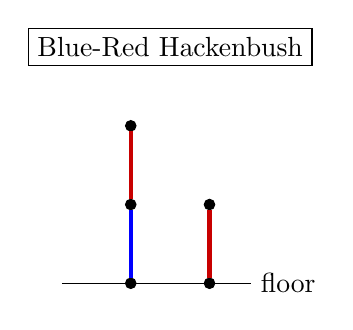
\begin{tikzpicture}
	\node[draw] (title) at (1.5, 3) {Blue-Red Hackenbush};
	\node (p1) at (0,0) {};
	\node (p2) at (3,0) {floor};
	\begin{scope} [every node/.style={scale=0.4, circle, draw, fill=black}]
		\node (p3) at (1,0) {};
		\node (p4) at (1,1) {};
		\node (p5) at (1,2) {};
		\node (p6) at (2,0) {};
		\node (p7) at (2,1) {};
		\draw (p1) -- (p2);
		\begin{scope} [ultra thick]
			\draw[blue] (p3) -- (p4);
			\draw[red] (p4) -- (p5);
			\draw[red] (p6) -- (p7);
		\end{scope}
	\end{scope}
\end{tikzpicture}


In this game, a move is made by taking a single colored edge of the image and removing any edges that become disconnected from the floor. One player can only remove blue edges, and the other, red edges.

It is a common practice to assume that, unless specified otherwise, games will be played between the players \naming{Left (bLue)} and \naming{Right (Red)}.




% Theory
    \chapter{Theory}
    \textcolor{red}{This chapter should outline, compare and discuss key ideas, explanations, concepts, models and theories. You should present these ideas in a systematic, well-structured and logical sequence. It is expected that you use prominent and up-to-date books and articles. All literature should be referenced, not just for quotations, but also for ideas and information/knowledge drawn from the works of others.\\
Refer to the \href{http://libguides.lub.lu.se/plagiarism}{Teaching and Learning platform} for guidance on how to incorporate references into your text}

\section{Previous Research}
Lorem ipsum dolor sit amet, consectetur adipiscing elit. Duis ut ipsum nec orci interdum sollicitudin ut eu nunc. Pellentesque ultricies eros in justo sagittis, eget blandit velit aliquet. Aenean ac lectus nibh. Quisque ac est pellentesque, ullamcorper sem sit amet, pharetra quam. Morbi ullamcorper placerat diam, sed tincidunt odio.

\section{Theoretical Approach}
Lorem ipsum dolor sit amet, consectetur adipiscing elit. Duis ut ipsum nec orci interdum sollicitudin ut eu nunc. Pellentesque ultricies eros in justo sagittis, eget blandit velit aliquet. Aenean ac lectus nibh. Quisque ac est pellentesque, ullamcorper sem sit amet, pharetra quam. Morbi ullamcorper placerat diam, sed tincidunt odio.

    
% Data
    \chapter{Data}
    \textcolor{red}{This Chapter should demonstrate that you have conducted a thorough and critical investigation of relevant sources.
Apart from a presentation of the sources of your data, this chapter allows you to critically discuss the data (whatever these data are, ‘quantitative’ or ‘qualitative’, primary or secondary), which is proof of good research. You can even do good research with poor data but you must demonstrate that you are aware of the data quality and accordingly are careful in your interpretations. Essentially, there are three aspects to consider:
\begin{enumerate}
\item	Reliability, which, for example, could depend on whether they are estimates or more direct evidence;
\item	Representativity, which is about how typical the data are; for example, you may have arguments why the very few cases are typical or you may carry out statistical tests;
\item Validity, which is about the relevance of the data for your case. Strictly speaking, sometimes no valid data are available but one may argue that there are other data which could be used as ‘proxies’.) 
\end{enumerate}
}
\section{Source Material}
Lorem ipsum dolor sit amet, consectetur adipiscing elit. Duis ut ipsum nec orci interdum sollicitudin ut eu nunc. Pellentesque ultricies eros in justo sagittis, eget blandit velit aliquet. Aenean ac lectus nibh. Quisque ac est pellentesque, ullamcorper sem sit amet, pharetra quam. Morbi ullamcorper placerat diam, sed tincidunt odio.
    
% Methods
    \chapter{Methods}
    \textcolor{red}{In this Chapter, you present in more concrete terms the method(s) you are going to apply. And as always in research, it is good to demonstrate awareness of the weaknesses or limitations of the method you use. It makes no difference if you work with interviews, econometric models, or a comprehensive analysis of data from various sources. Transparency should be the guideline: make it possible for your readers to follow, or even repeat, your analysis!}

\section{The Approach [or Model]}
Lorem ipsum dolor sit amet, consectetur adipiscing elit. Duis ut ipsum nec orci interdum sollicitudin ut eu nunc. Pellentesque ultricies eros in justo sagittis, eget blandit velit aliquet. Aenean ac lectus nibh. Quisque ac est pellentesque, ullamcorper sem sit amet, pharetra quam. Morbi ullamcorper placerat diam, sed tincidunt odio.
    
% Empirical Analysis
    \chapter{Empirical Analysis}
    \textcolor{red}{This chapter covers three areas: analysis of the data; discussion of the results of the analysis; and how your findings relate to the literature. The analysis of the data can be discussed here but the details of any analysis, such as statistical calculations, should be shown in the appendices. You should present any discussion clearly and logically and it should be relevant to your research questions/hypotheses or aims and objectives. Insert any tables or figures that you decide are important in a relevant part of the text not in the appendices, and discuss them fully. Make sure that you relate the findings of your primary research to your literature review. You can do this by comparison: discussing similarities and particularly differences. If you think your findings have confirmed some literature findings, say so and say why. If you think your findings are at variance with the literature, say so and say why.}
\section{Results}
Lorem ipsum dolor sit amet, consectetur adipiscing elit. Duis ut ipsum nec orci interdum sollicitudin ut eu nunc. Pellentesque ultricies eros in justo sagittis, eget blandit velit aliquet. Aenean ac lectus nibh. Quisque ac est pellentesque, ullamcorper sem sit amet, pharetra quam. Morbi ullamcorper placerat diam, sed tincidunt odio.

\textcolor{red}{When placing tables (\autoref{tab:econ}) within the body of the text, the citation is placed above the table.} 


\vfill

\newpage 

\section{Discussion}
Lorem ipsum dolor sit amet, consectetur adipiscing elit. Duis ut ipsum nec orci interdum sollicitudin ut eu nunc. Pellentesque ultricies eros in justo sagittis, eget blandit velit aliquet. Aenean ac lectus nibh. Quisque ac est pellentesque, ullamcorper sem sit amet, pharetra quam. Morbi ullamcorper placerat diam, sed tincidunt odio.

\textcolor{red}{When placing figures (illustrations, pictures, graphs, diagrams, charts, maps etc.) within the body of the text, the citation is placed below the figure (\autoref{fig:moun})}


    
% Conclusion
    \chapter{Conclusion}
    Combinatorial game theory is a new field in mathematics that was initially found in the blend of recreational mathematics, combinatorics and number theory. While the initial focus is finding strategies to play better and win games, the developments it prompted in other areas of mathematics have their own place, independent of the initial purpose. The Surreal Numbers form a class with many interesting properties and found much enthusiasm for that reason, not because it was necessary to analyze games.

However, the surreal numbers inevitably carry the simplicity inherited from the mathematical plays it was created/discovered for. It is commonplace to learn how to breach the gap between rational and real numbers only in superior education, partially because any of the common constructions involves operations and procedures not used in school. Surreal Numbers give for free the construction of real numbers from its few and simple rules. Not only the reals, but a definition of positivity and negativity that dismisses comparison, a common method for the creation of all the numbers, new numbers and, at last, a direct way of visualizing each number with RB-Hackenbush games. Numbers are the main building block the text used to analyze games.

The non-numbers, a name used in this text for games with temperatures, are the remaining games and required more elements and concepts to be understood. The thermograph, or the form commonly used to visualize temperature, options, stops and boiling points, is extensively analyzed and the text presents one of the most recent related results.

The reader that understands all the featured topics and is able to replicate calculations and results to games other than the mentioned might carry the false belief that understands all of combinatorial game theory. This text, however, only describes the class of partisan games leaving many variations even unmentioned. Not only the focus is specific, but also not all perspectives necessary to tackle the problem of finding the best move are visited.

These information serves to show that there is much more to the field, not that little progress understanding it was made. In fact, it is fair to state that the classes of games discussed in the text are the more complicated ones and many of the definitions apply to other classes.

Both in the results discussed and the ones omitted there is a common trend in this field. The definitions are always simple, but powerful enough to allow many questions, and, although there are many open questions, the proofs are and solutions are simple as well. The procedure to build all dyadic rationals in domineering boards, for example, is based on a theorem provable in two lines of text and applying it is the simplest of ways. Although its explanation is simple, it remained open for years and the resulting pattern is not something that would be found before the proof.

Finding the upper bound to temperature is another case where the question remained open for long, but the strategy used to answer is simplicity: it consists only of listing and manipulating properties of the thermographs.That is not to say that the bounding of temperature is completely solved but the progress made used simple steps.

From this perspective combinatorial game theory is a beautiful field in mathematics. The definitions it is based upon are extremely few in number and very simple in form, but they allow proving more complex problems in a uncomplicated manner. However, in this text, one of the unvisited places in the field is computational complexity. In practice, calculating values is not an easy problem.

The other featured aspect skipped is the variety of forms combinatorial games might take, because the text only deals with partisan games played on normal conditions. The remaining contains a brief description of these two skipped problems and points toward texts on th respective subjects. This chapter, that finalizes the text, also addresses a few of the next steps studying or researching the field and ends with a personal reflection on the learning, implementing and writing experiences involved in this work.


\subsection*{Undeveloped Pieces}

\subsubsection*{Complexity}

The text repeatedly made the case that most concepts are simple in Combinatorial Game Theory. It said, for example, that the method used to find the number a game is equal to is straight-forward. However this hides an important factor.

Either calculating the number or building a thermograph requires, first, traversing the game tree. Traversing this tree and calculating the values is simple enough, but it is slow. And it is slow because this tree quickly becomes large. For example, consider the following game of Domineering.

\begin{center}

\begin{tikzpicture}
\draw[step=0.5cm,color=gray] (-1,-1) grid (1,1);
\newcounter{mycount}
\setcounter{mycount}{`A}
\foreach \y in {+0.75,+0.25,-0.25,-0.75}
\foreach \x in {-0.75,-0.25,0.25,0.75}
\node at (\x,\y) {\addtocounter{mycount}{1}};
\end{tikzpicture}
\end{center}

There are, of course, 25 squares, which means that at most 12 moves might be made and in addition, some of these moves might be equivalent, so they do not have to be computed multiple times. It happens that only 604 nodes, or different position, may be reached\cite{1}. In a $6\times 6$ board it jumps to $17,232$ and in $7\times 7$ and $8\times 8$ board it goes to $408,260$ and $441,990,070$ nodes. Although these results are from 1998, results on larger boards took many years and only in 2016 a result for $11 \times 11$\cite{2} board was found, but abandoning a naive building of a game tree. The game tree of a $9\times 9$ board has around 25 trillion nodes.

If not clear at first it should be now that there is no known form of calculating values for games in polynomial time is respect to their sizes. The question, then, is in what class of problems it fits. It happens that many of the games are known to be PSPACE-complete and some are known to be EXPTIME.

There is of course much more to be said an it is another very interesting topic. A good starting point is \textit{Playing Games with Algorithms: Algorithmic Combinatorial Game Theory}\cite{3}. The thesis \textit{Games, Puzzles, and Computation} is more extensive, covering different classes of games, but may be more complex. Regardless of the suggested texts, there is a large amount of great books on complexity theory.

\subsubsection*{Other games}

By looking at the definition of combinatorial games given in the beginning of section 2, it is easy to come up with games that do not fit well the class of games studied, the short games. One clear example is the game of chess, because there are ties and there are drawn positions.

However, games like chess are not the only class of games that behave differently. Consider G-Hackenbush, a variation of RB-Hackenbush, in which both blue and red edges are replaced by green ones. Green edges may be removed by either player, meaning that both players have the same available moves regardless of the position. The class of games that follow this property is called Impartial Games.

Impartial games were the first games studied, previously to the consolidation of the modern form of the field. They have an interesting property of being reducible to an instance of a game of Nim. 

Games like chess, on the other hand, are not so simple. there are more classes of results than short games, which allows games to become more complex. Such games benefit from knowing short game's theory but do require further concepts. A good place to start is the corresponding chapter in the book \textit{Combinatorial Game Theory}.


\subsection*{Post-Match}

The choice of Combinatorial Game Theory as subject was an extremely fortunate decision. This field triggered the feeling of uncovering something beautiful hidden in plain sight. I believe the book \textit{Winning Ways} played a role in that due to the presentation I became found of, but I do considered there is inherent beauty in the field.

I believe the simplicity of everything about it is something to awe. This is the most important reason why this thesis ended up being about it and not some other subject. The first step in this directions was a great interest in the games of Chess, Shogi and Go. The first idea I had was to develop heuristics to find shortest paths in the game of chess, and possibly extend that to other games using more general graph theory.

During this period I started reading articles and scrolling through books and that quick led me into the field of Combinatorial Game Theory. The book \textit{Winning Ways} is one of the canonical references and I luckily started with that. This choice led me to a year of great learning experiences, in many areas, and personal maturing.

Learning and writing about the topics of this text was the most important activity to conclude my Bachelor's Thesis, but there are other subjects I studied in the process that went unmentioned in the text. I am grateful for those too, as I got to develop my understanding of real analysis and complexity theory further than I would normally, for example. This year was also the one of we had the corona virus widespread and, hopefully, the last year we have to partake isolation and health/economic insecurity.

I had only handful of on-campus classes and that required me, and most of the world, to adapt to new circumstances. While it did not effect the content of this text directly, it greatly impacted the world we live in. Frequently during the year I found myself struggling to concentrate and in a general bad mental state. The consistent work it took really helped keeping me on track. Another factor that can not go unmentioned is the help of my advisor.

José Coelho kept regularly meeting me almost every week during this year. That helped a lot keeping me in check and I am extremely thankful of the dozens of hours we spent talking and discussing the most varied subjects. In the times I did not have work to show he was understanding and his willingness to help pushed me further and further.












    
% Bibliography
    \phantomsection
    \addcontentsline{toc}{chapter}{References}%
    \bibliography{bibliography}
    
    \vspace{2.0cm}
    \textcolor{red}{Refer to \href{http://libguides.lub.lu.se/plagiarism}{LUSEM’s Harvard referencing guidelines} in the Teaching and Learning platform. \url{Lusem.lu.se/asks}}
    % The template provides \hcite and \mcite commands to present hyperlinked references in the 
    % Harvard referencing style '(Author, Year)'  and 'Author (Year)'
    % The template has an automated bibliography section based on references 
    % consistent with entries in the 'bibliography.bib' file 

% Appendices
    \appendix
    \chapter{(Appendix A title)}
    \textcolor{red}{The final sections of your thesis are the appendices. Each appendix should be lettered (A, B, etc.,) and should consist of detailed information that is interesting but not essential to the main thrust of your findings section.\\
The appendices should be in the order that they are referred to in the main text. For instance, if Appendix A refers to something on page 25 and Appendix B refers to something on page 15, the appendices need to be re-lettered. This inconsistency occurs when text is moved around or inserted.)}

    
     \chapter{(Appendix B title)}
    \input{sections/appendix_B}

\end{document}
%----------------------------------------------------------------------------------------------------%
